\part{Inheritance and polymorphism}
\frame{\partpage}

\begin{frame}[fragile]{Different shapes}
	\pause Handling of multiple shapes is currently not ideal
	\begin{itemize}
		\pause\item \lstinline{draw} method has a big \lstinline{if}-\lstinline{elif} block
		\pause\item Imagine if we also had to do e.g.\ collision detection -- we'd need another \lstinline{if}-\lstinline{elif} block
		\pause\item If we add a new shape, we have to remember to update all of these blocks
	\end{itemize}
\end{frame}

\begin{frame}{A better way?}
	\begin{itemize}
		\pause\item We could define multiple classes, e.g.\ \lstinline{SquareBall}, \lstinline{CircleBall}, \lstinline{TriangleBall}
		\pause\item But they would have common code (e.g.\ \lstinline{update} method) that we would need to copy and paste...
	\end{itemize}
\end{frame}

\begin{frame}[fragile]{Inheritance}
	\begin{itemize}
		\pause\item Classes can \textbf{inherit} from other classes
	\end{itemize}
	\begin{lstlisting}
class SquareBall(Ball):
	def __init__(self):
		...
	\end{lstlisting}
	\begin{itemize}
		\pause\item Here \lstinline{Ball} is the \textbf{base class}, \lstinline{SquareBall} is the \textbf{derived class} or \textbf{subclass}
		\pause\item The subclass automatically has all fields and methods from the base class
		\pause\item The subclass can add new fields and methods
		\pause\item The subclass can also \textbf{override} methods from the base class
	\end{itemize}
\end{frame}

\begin{frame}{Live coding}
\end{frame}

\begin{frame}{Inheritance hierarchy}
	\begin{columns}
		\pause
		\begin{column}{0.3\textwidth}
			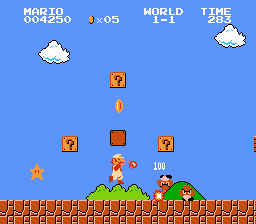
\includegraphics[width=\textwidth]{mario}
		\end{column}
		\pause
		\begin{column}{0.68\textwidth}
			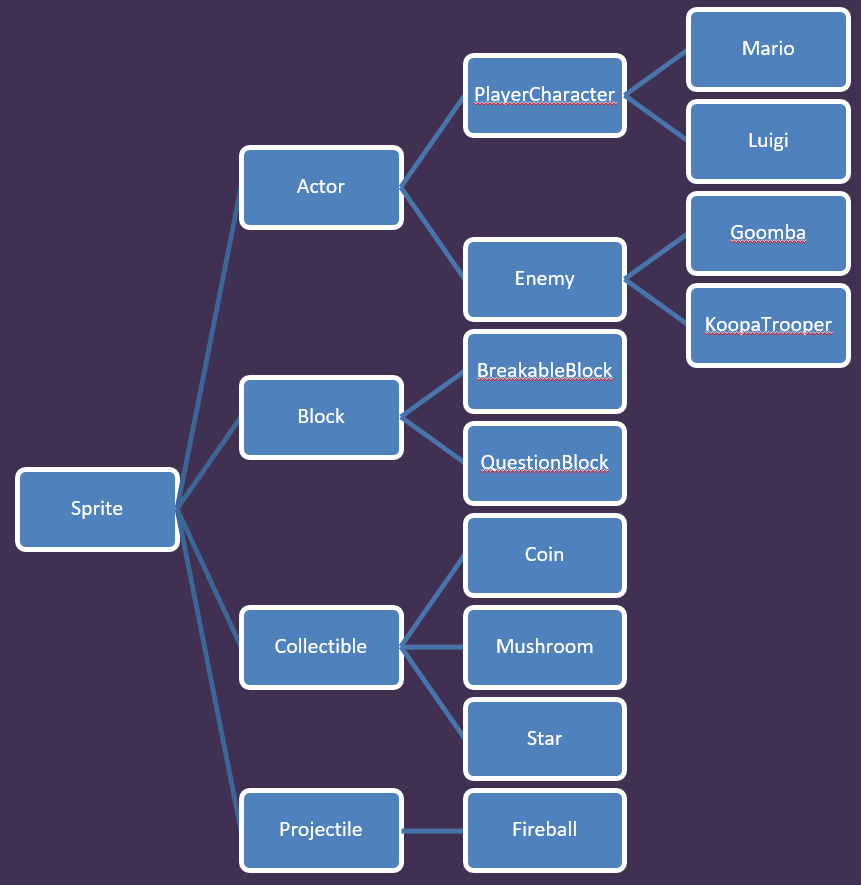
\includegraphics[width=\textwidth]{hierarchy}
		\end{column}
	\end{columns}
\end{frame}

\begin{frame}[fragile]{Polymorphism}
	\begin{lstlisting}
ball.draw(screen)
	\end{lstlisting}
	\begin{itemize}
		\pause\item Here \lstinline{ball} might be an instance of \lstinline{SquareBall}, \lstinline{CircleBall} or \lstinline{TriangleBall}
		\pause\item Whichever it is, Python will execute the appropriate \lstinline{draw} method
		\pause\item The author of this code doesn't need to worry about squares, circles or triangles
		\pause\item If we added a new shape class, everything works automatically
		\pause\item This is \textbf{polymorphism} --- the same code can use objects of many different classes
			\begin{itemize}
				\pause\item From Greek: ``many-shape-ism''
			\end{itemize}
	\end{itemize}
\end{frame}

\begin{frame}[fragile]{Abstract classes and methods}
	\begin{itemize}
		\pause\item It no longer makes sense to instantiate \lstinline{Ball} directly --- it exists only as a base class for other classes
		\pause\item \lstinline{Ball} is an \textbf{abstract class}
		\pause\item Similarly, \lstinline{Ball.draw()} should never be called directly --- all subclasses should override it
		\pause\item \lstinline{Ball.draw()} is an \textbf{abstract method}
	\end{itemize}
\end{frame}

